\documentclass[a4paper,12pt]{article}

\usepackage[14pt]{extsizes}
\usepackage{cmap}					% поиск в PDF
\usepackage{mathtext} 				% русские буквы в формулах
\usepackage[T2A]{fontenc}			% кодировка
\usepackage[utf8]{inputenc}			% кодировка исходного текста
\usepackage[english,russian]{babel}	% локализация и переносы
\usepackage{graphicx}
\usepackage{geometry}
\usepackage{amsmath}
\usepackage[table]{xcolor}
\setlength\extrarowheight{2pt}


\geometry{verbose, a4paper, tmargin=2cm, bmargin=2cm, lmargin=3cm, rmargin=2cm}
\author{Vysotsky Maxim}
\title{Отчёт}
\date{2022}

\begin{document}
	\begin{titlepage}
		\begin{center}
			{Министерство науки и высшего образования Российской Федерации
				НАЦИОНАЛЬНЫЙ ИССЛЕДОВАТЕЛЬСКИЙ ТОМСКИЙ
				ГОСУДАРСТВЕННЫЙ УНИВЕРСИТЕТ (НИ ТГУ)}
		\end{center}
		\begin{center}
			{Физический факультет}
		\end{center}
		
		
		\vspace{8cm}
		{
			\begin{center}
				{\bf Лабораторная работа №1-8}\\
				Определение теплоёмкости твёрдых тел калориметрическим методом
			\end{center}
		}
		\vspace{2cm}
		\begin{flushright}
			{Руководитель:\\ канд. физ.-мат. наук\\
				Конов И. А. \\
				Работу выполнили:\\
				Левин Н. Н. \\
				Высоцкий М. Ю.\\
				\vspace{0.2cm}
				гр. 052101}
		\end{flushright}
		\vspace{3cm}
		\begin{center}
			Томск, 2022
		\end{center}
	\end{titlepage}

\section{Теоретическое введение}
\textbf{Цель работы:} определение теплоёмкости образцов металлов калориметрическим методом с  использованием электрического нагрева.

\subsection{Теория метода. Закон Дюлонга -- Пти. Закон Джоуля -- Коппа}
\hspace{\parindent}Из теории идеального газа известно, что средняя кинетическая энергия, приходящаяся на одну степень свободы молекулы, равна:
$$ \langle \varepsilon_i \rangle = \frac{1}{2}kT$$

Тогда среднее значение полной энергии частицы при колебательном движении в узлах кристаллической решётки будет равна:
$$ \varepsilon = 3\bigg(\frac{kT}{2} + \frac{kT}{2}\bigg) = 3kT$$

Здесь учитывается факт, что атом в кристалле имеет три колебательные степени свободы, и на каждую приходится энергия, равная $kT$ (по $\frac{kT}{2}$ на кинетическую и потенциальную соответственно).

Полную энергию одного моля газа можно найти, помножив среднюю энергию одной частицы на число Авогадро:
\begin{equation}\label{energy}
U_{\mu} = \varepsilon N_A = 3kN_AT = 3RT,
\end{equation}
где $R$ -- универсальная газовая постоянная, равна 8,314 $\frac{Дж}{моль*K}$.

Так как теплоёмкости $C_V$ и $C_P$ мало различимы для твердых тел, в следствие малого коэффициента теплового расширения, молярная теплоёмкость твердого тела будет равна:
\begin{equation}\label{Dulong-Pti}
C_\mu = \frac{\partial U_\mu}{\partial T} = 3R = 29,94 \hspace{0.2cm} \frac{Дж}{моль*K}
\end{equation}

Выражение \eqref{Dulong-Pti} называется \textbf{законом Дюлонга и Пти}.

Для химических соединений справедлив закон Джоуля -- Коппа - закон, описывающий теплоёмкость сложных (состоящих из нескольких химических элементов) кристаллических тел. Он основан на законе \eqref{Dulong-Pti}. 

Формулировка закона такова: Каждый атом в молекуле имеет три колебательных степени свободы и обладает энергией $\varepsilon = 3kT$. Соответственно, молекула из n атомов обладает в  n раз большей энергией: 
$$\varepsilon = 3nkN_A = 3nR$$
Иными словами, \textit{молярная теплоёмкость вещества равна сумме теплоёмкостей составляющих его химических элементов}. Важно отметить, что закон Джоуля -- Коппа выполняется даже для кристаллов, содержащих в своей структуре не подчиняющиеся закону Дюлонга -- Пти химические элементы. 

При $T \rightarrow 0$, теплоёмкость также $C \rightarrow 0$. Вблизи абсолютного нуля, $C_\mu$ всех тел пропорциональна $T^3$. И лишь при достаточного высокой температуре, характерной для каждого вещества, начинает выполняться закон \eqref{Dulong-Pti}. Данную особенность теплоёмкостей твердых тел при низких температурах описывают \textbf{квантовой теории теплоёмкости Эйштейна и Дебая}.

\subsection{Калориметрический метод}
\vspace{\parindent} Для экспериментального определения теплоёмкости исследуемое тело помещается в калориметр, нагреваемый электрическим током. Если температуру калориметра (без образца) медленно увеличивать, то энергия тока за время $\tau$ пойдет на нагревание пустого калориметра. Выполняется закон сохранения энергии:
\begin{equation}\label{Ein-Deb}
IU_\tau = m_0c_0T + \Delta Q,
\end{equation}
где $I, U$ ток и напряжение нагревателя, $\tau$ - время нагревания, $m_0$ - масса пустого калориметра, $c_0$ - удельная теплоемкость пустого калориметра, $\Delta Q$ - потери тепла в теплоизоляцию калориметра и в окружающее пространство.
Выразив $\tau$ из \eqref{Ein-Deb} и построив график зависимости $\tau(T)$, мы увидим, что тангенс угла наклона этой зависимости
$$\tau = \frac{m_0c_0}{IU}T + \frac{\Delta Q}{IU}$$
\begin{equation}\label{empty}
tg(\alpha_0) = K_0 = \frac{m_0c_0}{IU} = \frac{C_0}{IU}
\end{equation}
позвляет нам найти теплоёмкость пустого калориметра: 
$$C_0 = K_0IU$$

Нагревая калориметр с образцом внутри, мы можем снова записать закон сохранения энергии:
\begin{equation}\label{obrazets}
IU\tau_0 = m_0c_0\Delta T + mc\Delta T + \Delta Q,
\end{equation}
где $m$ - масса образца, $c$ - удельная теплоёмкость образца.

Также выразив $\tau$ из \eqref{obrazets} и построив график, увидим, что у угловой коэффициент также связан с теплоёмкостью, только в этом случае - теплоёмкостью образца:
$$\tau = \frac{m_0c_0 + mc}{IU}T + \frac{\Delta Q}{IU}$$
\begin{equation}\label{not_empty}
tg(\alpha) = K = \frac{m_0c_0 + mc}{IU}T  = \frac{C_0+mc}{IU}
\end{equation}
Из \eqref{empty} и \eqref{not_empty} получим выражения для удельной и молярной теплоёмкости образца:
\begin{equation}
KIU - C_0 = mc = C; c = \frac{KIU - C_0}{m}
\end{equation}
\begin{equation}
C_\mu = c*\mu = \frac{(KIU - C_0)\mu}{m}
\end{equation}

\section{Ход эксперимента}
\hspace{\parindent}Для определения теплоёмкостей представленных образцов мы пользовались калориметром. Для начала мы понизили температуру рабочей области установки посредством помещения в неё целофанового пакета со снегом. После установления температуры на отметке $35^\circ С$, мы начали нагревать пустой калориметр посредством включения соответствующего тумблера на установке, предварительно выставив значения напряжения и силы тока соответственно: $U$ = 15 В; $I$ = 0,6 A.

Вышеперечисленная последовательность действий была произведена повторно для двух образцов: дюраль и латунь.
\begin{center}
	\resizebox{\textwidth}{!}{
	\begin{tabular}{|c|c|c|c|c|c|c|c|c|c|c|}
		
		\hline
		Образец&	$t_1, c$&	$t_2, c$&	$t_3, c$&	$t_4, c$&	$t_5, c$&	$t_6, c$&	$t_7, c$&	$t_8, c$&	$t_{ср}, c$& $t_{общ}, c$
		\\
		\hline
		Пустой&	13,83&	13,71&	12,1&	11,32&	10,23&	10,85&	10,74&	9,75&	11,56625&	92,53
		\\
		Дюраль&	13,38&	12,43&	11,46&	10,79&	12,42&	10,28&	11,89&	12,56&	11,90125&	95,21
		\\
		Латунь&	11,92&	11,49&	11,51&	11,52&	10,95&	11,84&	11,18&	8,84&	11,15625&	89,25
		\\
		\hline		
		
	\end{tabular}
	}
\end{center}


\begin{center}
	\begin{tabular}{|c|c|c|}
		\hline
		Образец&	Масса образца, кг& Атомная масса, $\frac{кг}{моль}$
		\\
		\hline
		Дюраль&	0,04621& $26,98*10^-3$
		\\
		Латунь&	0,13857& $63,57*10^-3$
		\\
		\hline		
	\end{tabular}
\end{center}

\newpage
\hspace{\parindent}Используя полученные данные, мы построили три графика зависимости времени от температуры:
\begin{figure}[h!]
	\begin{center}
		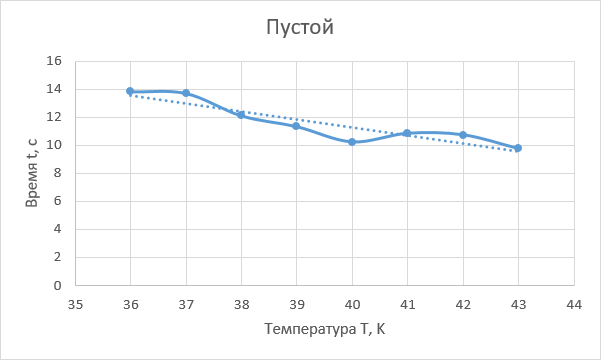
\includegraphics[scale=1]{1}
	\end{center}
	\caption{График зависимости t от T для пустого калориметра}
	
\end{figure}

\begin{figure}[h!]
	\begin{center}
		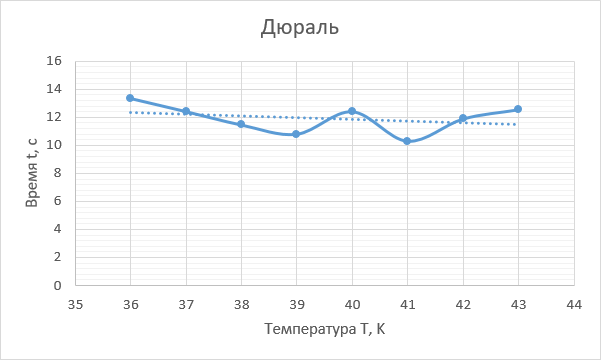
\includegraphics[scale=1]{2}
	\end{center}
	\caption{График зависимости t от T для дюралюминия}
	
\end{figure}

\newpage
\begin{figure}[h!]
	\begin{center}
		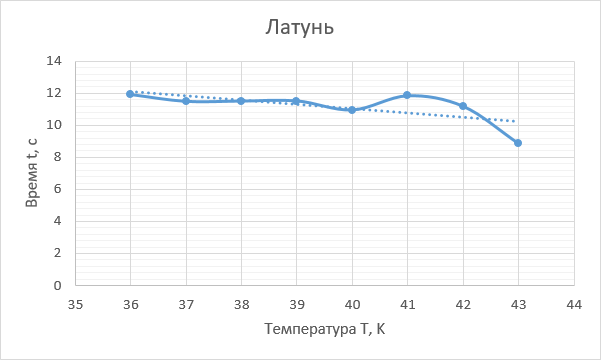
\includegraphics[scale=1]{3}
	\end{center}
	\caption{График зависимости t от T для латуни}
	
\end{figure}
\hspace{\parindent}Проанализировав полученные кривые, мы можем сказать, что в каждом конкретном случае образер нагревался неравномерно, что может быть связано с непостоянством отдачи тепла от нагревательного элемента калориметру.

Далее, по ходу работы, нам было необходимо определить тангенсы углов наклона полученных графиков. Для их нахождения мы использовали линии тренда, а также определение тангенса. Полученные значения для каждого из трех случаев представлены ниже:

\begin{center}
	\begin{tabular}{|c|c|}
		\hline
		Образец&	$tg(\alpha)$
		\\
		\hline
		Пустой&	11,56625
		\\
		Дюраль&	11,90125
		\\
		Латунь&	11,15625
		\\
		\hline		
	\end{tabular}

\end{center}

\newpage
\hspace{\parindent}После нахождения тангенса угла наклона мы определили $C_0$ из соотношения - $C_0 = K_0IU$, а также, используя формулы (7) и (8), $C_\mu$ и $c$ для дюрали и латуни соответственно:

$$C_0\pm\Delta C_0 = 104\pm1\frac{Дж}{с}$$


\begin{center}

	\begin{tabular}{|c|c|c|}
		\hline
		Образец&	$C_\mu \pm \Delta C_\mu, \frac{Дж}{моль*с}$&	$с \pm \Delta c, \frac{Дж}{кг*с}$
		\\
		\hline
		Дюраль&		$1,7\pm0,4$&	$65\pm13$
		\\
		Латунь&		$-1,6\pm0,3$&	$-26\pm4$
		\\
		\hline		
	
	\end{tabular}
\end{center}

\hspace{\parindent}Если принять, что измерения, последовательность действий и расчеты верны, то данные значения будут конечными в данной работе, т.к. указанные выше величины являются искомыми. Однако, у нас появились некоторые сомнения, касательно результатов полученных для латуни.

\hspace{\parindent}В следуещем пункте мы оценим погрешности измерений, а после попробуем разобраться в вызвавшем сомнения моменте.

\newpage
\section{Погрешности измерений}

\hspace{\parindent}Следуя рекомендациям из методических материалов, для определения погрешностей теплоемкостей мы будем учитывать систематические погрешности выставленных напряжения и силы тока, а также косвенные погрешности определенных с помощью графиков значений $K$ и $К_0$.

$$\Delta C_0 = \sqrt{\Delta K_0^2 + \Delta I^2 + \Delta U^2},$$
где $\Delta K_0$ = 0,125, $\Delta I$ = 0,01 А, $\Delta U$ = 1 В.

\vspace{10,25pt}
\hspace{\parindent}Откуда

$$\Delta C_0 = 1 \frac{Дж}{с}$$

\hspace{\parindent}Проведем идентичные действия для $\Delta KIU$:
$$\Delta KIU = 1,17 \frac{Дж}{с}$$

\hspace{\parindent}Далее, с помощью указанной в методических материалах формулы для определения $\Delta C$, найдем необходимую погрешность.

$$\Delta C = \sqrt{(\Delta KIU)^2-(\Delta C_0)^2}$$

\hspace{\parindent}Откуда

$$\Delta C = 0,6\frac{Дж}{с}$$

\hspace{\parindent}С помощью простых вычислений частных производных соответственно найдем $\Delta C_\mu$ и $\Delta c$.

$$\Delta c_1 = 13 \frac{Дж}{кг*с};$$

$$\Delta c_2 = 4 \frac{Дж}{кг*с};$$

$$\Delta C_{\mu1} = 0,4 \frac{Дж}{моль*с};$$

$$\Delta C_{\mu2} = 0,3 \frac{Дж}{моль*с},$$

где $\Delta c_1$ и $\Delta c_2$ - косвенные погрешности для удельных теплоемкостей дюрали и латуни соответственно, $\Delta C_{\mu1}$ и $\Delta C_{\mu2}$ - косвенные погрешности для молярных теплоемкостей дюрали и латуни соответственно.

\newpage
\section{Вывод}
\hspace{\parindent}Даже с учетом погрешностей, полученные для латуни теплоемкости остаются среди отрицательных значений. Это говорит о том, следуя определению теплоемкости, что в данном случае при подведении тепла к образцу, температура уменьшается.

Заинтересованные данным фактом, мы изучили некоторые открытые источники в интернете, связанные с данной темой. Оказалось, что данное явление отрицательной теплоемкости свойственно газам в некоторых специфических условиях, что не подходит в нашем случае, т.к. мы работаем с металлами.

Также следует заметить, что из полученных результатов наблюдается явное невыполнение закона Дюлонга-Пти, а также закона Джоуля-Коппа, т.к. в случае его выполнения множитель $n$ был бы дробным, что невозможно, потому что данный множитель обозначает количество атомов в молекуле вещества (очевидно, что данная величина не может быть дробной).

Учитывая вышесказанные заключения, было принято решение оценить выполнимость классического приближения, с точки зрения квантовой теории.

\hspace{\parindent}По принципу неопределенности Гейзенберга:
$$\Delta p_x \Delta a_x \gg \hbar,$$

где $\Delta p_x$ - импульс атома (характеризует кинетическую энергию), $\Delta a_x$ - отклонение атома от положения равновесия (потенциальная энергия), $\hbar$ - приведенная постоянная Планка.

Согласно теореме о распределении внутренней энергии, мы можем приравнять $\Delta p_x$ и $\Delta a_x$ к $\frac{1}{2}kT$ поочередно:

$$\Delta p_x = \frac{1}{2}kT$$
$$\Delta a_x = \frac{1}{2}kT$$

Откуда

$$<\Delta p_x> = \sqrt{mkT}$$
$$<\Delta a_x> = \sqrt{\frac{kT}{\alpha}}$$

\newpage
\hspace{\parindent}Перемножим получившиеся величины:
$$\Delta p_x \Delta a_x \widetilde{=} kT\sqrt{\frac{m}{\alpha}}$$

Или

$$kT \gg \hbar\omega,$$

где $\omega$ - частота колебаний атома около положения равновесия, $\alpha$ - коэффициент упругости.

Таким образом значение $T$ должно быть много больше некоторого значения $\theta = \frac{\hbar\omega}{k}$ - характерной температуры. Здесь $k$ - постоянная Больцмана.

Расчеты по данным формулам не привели к положительному результату, поэтому было рассмотрено представление данных рассуждений с помощью коэффициента изотермического сжатия $\gamma$. Представленное ниже соотношение выводится при рассмотрении упругой силы, действующей на один атом:

$$\alpha = \frac{3a}{\gamma}$$

Откуда

$$\omega = \sqrt{\frac{3a}{\gamma m}},$$

где $a$ - межатомное расстояние, $m$ - масса одного атома (в нашем случае молекулы).

Значение величины $a$ будет определяться равенством:
$$a = \sqrt[3]{\frac{m}{\rho}},$$

где $\rho$ - плотность вещества.

Таким образом для численной оценки $\theta$ нам понадобятся значения $\gamma, \rho, m$, которые представлены в таблице для каждого образца соответственно:

\begin{center}

	\begin{tabular}{|c|c|c|c|}
		
		\hline
		Образец&	$\gamma*10^-13, \frac{см^2}{дин}$& $\rho, \frac{г}{см^3}$& $m*10^-23, г$
		\\
		\hline
		Дюраль&	$14,6$& 2,8& 28,17
		\\
		Латунь&	$12,16$& 8,73& 21,39
		\\
		\hline		
		
	\end{tabular}
\end{center}

Все значения, представленные выше, были получены из соответствующих таблиц, найденных в интернете. Также, размерности дынных величин представлены в системе СГС для простоты вычислений.

После всех вышеперечисленных рассуждений и рассчетов, мы получили соответсвующие значения $\theta$ для каждого из образцов.

\begin{center}
		\begin{tabular}{|c|c|}
			
			\hline
			Образец&	$\theta, K$
			\\
			\hline
			Дюраль&	140,66
			\\
			Латунь&	139,74
			\\
			\hline		
			
		\end{tabular}
\end{center}

Таким образом, чтобы выполнялось классическое приближение, необходимо, чтобы температуры рассматриваемых образцов были выше, чем соответствующие характерные температуры, а именно:

$$T_1 > 140,66K$$
$$T_2 > 139,74K$$

Если перевести в шкалу Цельсия:

$$\bar t_1 > -132,34^\circ C$$
$$\bar t_2 > -133,26^\circ C$$

Если проанализировать получившиеся температуры, то можно сказать, что классические приближения начнут выполняться для обоих образцов примерно в одно и то же время (разность характерных температур равна порядка одного градуса).

Учитывая данное исследование, мы делаем вывод, что в данной лабораторной работе выполняются необходимые условия для справедливости классических приближений, однако ответ на поставленный в начале вывода вопрос, касательно отрицательной теплоемкости, так и не был найден.

Мы предполагаем, что объяснение данного явления может содержаться в более глубоких разделах квантовой механики, знаний о которых у нас пока что, к сожалению, нет.
\end{document}